Neutron star mergers probe the nature of matter at densities and temperatures far beyond those available in the laboratory. 
The observation of GW170817 confirmed that gravitational waves can yield meaningful insights into the structure of neutron stars, and hence on the equation of state of matter above nuclear density~\cite{TheLIGOScientific:2017qsa,De:2018uhw,Fattoyev:2017jql,Tews:2018iwm,Margalit:2017dij,Annala:2017llu,Raithel:2018ncd}. Combining gravitational-wave and electromagnetic observations of the first neutron star merger with nuclear theory and numerical simulations has already shed new light on the equation of state of dense matter~\cite{Capano:2019eae,Dietrich:2020efo,AlMamun21}.
The ability of multi-messenger observations of merging neutron stars to
explore nuclear physics is determined by: the signal-to-noise ratio of the observed
gravitational-wave signals; the fidelity of the waveforms used 
to model gravitational-wave signals; the ability to model and extract 
information from electromagnetic counterparts; and
theoretical modeling of hot and cold dense nuclear matter and its 
connection to the observed quantities. In this chapter, we focus on the impact that the signal-to-noise
ratio of the signal has on the ability to measure the neutron star equation of state with current and future gravitational-wave detectors.

Gravitational-wave observations of binary neutron star mergers measure the nuclear equation of state through the star's tidal deformability $\Lambda$ which is imprinted on the phasing of the inspiral waveform. This measurement of $\Lambda$ is equivalent to a measurement of the neutron star radius, and hence the nuclear equation of state which connects these two quantities for a given mass. Previous studies have shown that Advanced LIGO will be able to measure the radius of a 1.4\msun~neutron star $R_{1.4}$ to better than 10\% precision with the first few tens of binary neutron star signals. However many plausible equations of state produce similar radii for a range of masses, so that distinguishing between them would require measurement precision better than 2\%. In this work we assess the ability of both Advanced LIGO and the proposed third-generation detector Cosmic Explorer, to make a precise measurement of the equation of state from a large population of simulated binary neutron star signals, for several equations of state that span the plausible range. We perform full Bayesian parameter estimation on all simulated signals and produce a combined measurement of $R_{1.4}$. We find that with 321 signals Advanced LIGO is able to measure $R_{1.4}$ to better than 2\% across the entire range of plausible equations of state, although the probability of seeing so many signals in the next decade is low. On the other hand we find that with one year of observation, Cosmic Explorer will be able to measure $R_{1.4}$ to within 0.6\% for a soft equation of state, and to within 0.15\% for a moderately stiff equation of state.

\section{Introduction}
The observation of the binary neutron star merger GW170817 during the second observing run of the LIGO-Virgo network provided the first constraints on the cold dense matter equation of state through gravitational waves~\cite{LIGOScientific:2017vwq}. The observations of AT2017gfo, the electromagnetic counterpart to GW170817, were also able to constrain the equation of state through estimates of the ejecta mass and velocity~\cite{Radice:2018ozg}, and by probing the fate of the merger remnant~\cite{Margalit:2019dpi}. Additional constraints have also recently come from pulsar observations and nuclear experiment: X-ray observations by the \textit{NICER} instrument of the pulsars J0740$+$6620 and J0030$+$0451 have mapped out some of the neutron star mass-radius relationship through direct radius measurements~\cite{Riley:2019yda,Riley:2021pdl,Miller:2021qha}, and in the low pressure regime the \textit{PREX-II} experiment has made precise measurements of the density dependence of the nuclear symmetry energy for lead atoms~\cite{PREX:2021umo}, which can be mapped to the higher pressures in neutron stars in order to also provide an estimate of the expected neutron star radius~\cite{Reed:2021nqk}. Recent efforts have been made to combine some of these and other disparate measurements into a generalized constraint on the equation of state, often given in terms of the radius of a 1.4\msun~neutron star $R_{1.4}$: \cite{Reed:2021nqk} combined the \textit{PREX-II} measurement and the \textit{NICER} constraints on the radius of the pulsar J0030$+$0451 to give $13.25~\mathrm{km}<R_{1.4}<14.26~\mathrm{km}$ (1$\sigma$ limits), and \cite{Al-Mamun:2020vzu} combined GW170817, quiescent low-mass X-ray binaries, photospheric radius expansion X-ray bursts, and J0030$+$0451 to find $R_{1.4}=11.83_{-0.71}^{+0.62}$~km (2$\sigma$ limits).

% P2 negative on current constraints
While great strides have been made in producing constraints on the equation of state, the prospects for improving these constraints using binary merger events still face significant challenges. GW170817 was a remarkably loud signal, with a signal-to-noise ratio of over 33, and yet the gravitational-wave observation alone was insufficient to conclusively distinguish the signal from a pair of merging black holes~\cite{LIGOScientific:2017vwq}. A second binary neutron star signal, GW190425, was observed by the LIGO-Virgo network but at a much lower signal-to-noise ratio of 13, which provided negligible information about the equation of state and also meant that no electromagnetic counterpart was identified~\cite{LIGOScientific:2020aai}. Similarly, there have been three gravitational-wave observations of probable neutron star--black hole mergers to date containing no measurable information on the equation of state, or any identifiable electromagnetic counterpart from the possible disruption of the neutron star~\cite{LIGOScientific:2020zkf,LIGOScientific:2021qlt}. Further complicating matters, the estimated merger rate of binary neutron stars in the local universe has been revised significantly lower after the completion of LIGO's third observing run~\cite{Abbott:2020gyp}, which means a correspondingly lower probability that future observing runs will produce a large set of observed signals that can be combined into a precise constraint on the equation of state.

% Add that SQM3, WFF2, and APR4 predict similar R_1.4 
Where previous works have investigated distinguishability between equation of state models, most have primarily focused on distinguishing models that differ substantially from one another. However many models exist that are consistent with current constraints but make similar predictions. As an example, the commonly used models WFF2, APR4, and SQM3, predict values for $R_{1.4}$ of 11.16, 11.32, and 11.37 kilometers, respectively. Naturally the prospect of distinguishing between these or other similar models is a much greater challenge, but this is very likely what will be required of future equation of state constraints. For the example models given, this will require measurements of $R_{1.4}$ with a precision better than 2\%.

% P3 why soft EOS is hard
The ability to measure the equation of state in gravitational-wave signals depends very sensitively on the equation of state itself, because the range of plausible models predict varying amounts of information in an inspiral waveform. Gravitational-wave signals from coalescing neutron stars carry information about the equation of state as a result of the tidal deformation that the stars' gravitational fields produce in one another. Specifically, the quadrupole moment $Q_{ij}$ of one neutron star is related to the tidal field $\mathcal{E}_{ij}$ of the other neutron star according to $Q_{ij} = -\lambda\mathcal{E}_{ij}$, where $\lambda$ is the tidal deformability of the neutron star~\cite{Flanagan:2007ix}. The tidal deformability is dependent on the equation of state and is commonly expressed in dimensionless form as
\begin{equation}
    \Lambda=\frac{2}{3}k_{2}\left(\frac{Rc^{2}}{Gm}\right)^5
\end{equation}
where $k_{2}$ is the tidal Love number. $R$ and $m$ are the radius and mass of the neutron star, respectively. The energy expended in deforming the stars results in a phase difference in the gravitational waveform as compared to a signal with non-deforming bodies. An equation of state that has a large $\Lambda$ for a given mass is said to be ``stiff", and will generally correspond to a larger radius as the neutron star is more able to hold itself up against gravity. A stiff equation of state produces a larger effect on the gravitational-wave phasing and is therefore more measurable. Conversely, a ``soft" equation of state will have a smaller $\Lambda$ and radius for a given mass, and produces a less measurable effect in a gravitational-wave signal.

% P4 lit review of forecasts
Given the difficulty of measuring the equation of state, an established method of improving constraints is to combine multiple observations in order to reduce statistical uncertainty~\cite{DelPozzo:2013ala}. Previous works have used various implementations of this method to estimate the measurability of the equation of state for a given signal population or detector network~\cite{DelPozzo:2013ala,Lackey:2014fwa,Agathos:2015uaa,Vivanco:2019qnt,Pacilio:2021jmq}. Lackey and Wade \cite{Lackey:2014fwa} combined signals in a simulated LIGO-Virgo network at design sensitivity, for several choices of equation of state. They constrain the neutron star radius across a range of masses and find that the radius can be measured to within $\pm1$ kilometer with 20 signals. Agathos {\it et al.}~\cite{Agathos:2015uaa} combined 200 signals in a LIGO-Virgo network and found that a catalog of at least 100 signals is sufficient to distinguish between soft, moderate, and stiff equations of state if one assumes perfect knowledge of the mass distribution, while 150 or more signals would be needed if the mass distribution was unknown. \cite{Vivanco:2019qnt} project that the 8 loudest signals from a population of 20 in a LIGO-Virgo network will constrain the radius of a canonical 1.4\msun neutron star to within 10\%. Pacilio {\it et al.}~\cite{Pacilio:2021jmq} combine 20 signals in both a LIGO-Virgo network and Einstein Telescope, a proposed third-generation detector. They find that LIGO-Virgo is unable to distinguish between similarly soft equations of state from a catalog of 12 used in the analysis, although Einstein Telescope can potentially make this distinction.

% P5 overview of results and method
In this chapter we build upon these previous works to produce an accurate forecast for a high precision measurement of the equation of state, using both a LIGO-Virgo network operating at design sensitivity as well as a planned third-generation detector Cosmic Explorer. We make our forecast using a population of simulated binary neutron star signals generated from astrophysically realistic parameter distributions. We produce parallel populations of these signals for three choices of equation of state that span the range of the most up-to-date constraints from gravitational-wave events, electromagnetic observations of pulsars and the kilonova AT2017gfo, and nuclear experiments. We perform full Bayesian parameter estimation for each signal in our populations to recover the intrinsic and extrinsic source parameters, and we use a collection of 2000 realistic equations of state built from nuclear theory as a prior distribution in our analysis. We produce a combined equation of state measurement across our populations by transforming each measurement to a constraint on $R_{1.4}$, the radius of a 1.4\msun~neutron star. We find that a LIGO-Virgo network is able to measure $R_{1.4}$ to within 2\% across the entire range of plausible equations of state, though a soft equation of state will require significantly more signals that are unlikely to occur within the next planned observing runs. We find also that an incorrect mass prior used by our LIGO-Virgo analysis introduces a bias in the equation of state measurement such that a combined measurement with better than 2\% precision will exclude the true equation of state at high confidence. We find that Cosmic Explorer is able to achieve better than 0.6\% precision on $R_{1.4}$ with signals representing one year of observations for even the softest equation of state in our analysis. We find that in our Cosmic Explorer analysis an incorrect mass prior did introduce a bias, although it was not large enough to strongly exclude the true equation of state even with the much smaller statistical uncertainty on the measurement.

% P6
The rest of this chapter is organized as follows: Section~\ref{sec:population} describes the simulated binary neutron star signals included in our analysis. In Section~\ref{sec:eos} we give background information on equation of state information in gravitational-wave inspiral signals and describe the equations of state used in this analysis. Section~\ref{sec:eos_meas_pe} gives details about our parameter estimation analysis including the method of combining measurements. Section~\ref{sec:eos_meas_results} presents the results of our analysis including constraints for each of our chosen equations of state. Finally, we conclude in Section~\ref{sec:eos_meas_conclusion}.

\section{Simulated signals}\label{sec:population}

To simulate measurement scenarios for a LIGO-Virgo network and Cosmic Explorer, we generate a population of simulated binary neutron star merger signals and project them onto the corresponding detectors. For LIGO-Virgo we simulate a three-detector network representing the LIGO Hanford, LIGO Livingston~\cite{TheLIGOScientific:2016agk,Buikema:2020dlj}, and Virgo~\cite{TheVirgo:2014hva} detectors. Each LIGO-Virgo detector is simulated at its design sensitivity by injecting simulated signals into Gaussian noise colored by the design power spectral density for each detector~\cite{Aasi:2013wya}. Cosmic Explorer is still in its design phase and does not have a final configuration or site location determined yet, although potential sites in the United States include locations in Utah or Idaho. For simplicity we use a hypothetical Cosmic Explorer detector at the same location and orientation as the LIGO Hanford detector. We choose the 40 kilometer arm length configuration optimized for detection of coalescing binaries for our analysis, and signals are injected into Gaussian noise colored by the corresponding design power spectral density~\cite{CE:NoiseCurves}.

% parameter distributions
Following the prescription of \cite{Agathos:2015uaa} we generate our simulated binary neutron star mergers using astrophysically motivated distributions for the source parameters. The collection of electromagnetic observations of known galactic pulsars has found their mass distribution to be well described by a Gaussian centered near 1.4\msun. However the gravitational wave observations of GW190425 and two of the neutron star--black hole signals show evidence for a greater number of high-mass neutron stars in the range $1.7-1.9$\msun. To account for both possibilities and to investigate the effect of a different mass distribution on the ability to measure the equation of state, we generate our population for two choices of mass distribution. For our primary population, source-frame component masses are drawn from a Gaussian distribution with mean $\mu_{m}=1.4$\msun~and standard deviation $\sigma_{m}=0.05$\msun. A secondary population has source-frame component masses drawn uniformly in the range $1-2$\msun. In all cases, component spins along the axis of orbital angular momentum are drawn from a Gaussian distribution with zero-mean and standard deviation $\sigma_{\chi}=0.02$. Sky locations are distributed uniformly across the sky, and the inclination and orientation of the binary systems is distributed uniformly on the sphere. For signals analyzed with the LIGO-Virgo network, distances are drawn uniformly in volume in the range [20, 585] Mpc, where the upper bound is the largest distance at which an optimally oriented binary merger with equal masses of 2\msun~would produce a single detector signal-to-noise ratio of 8. Simulated signals are then pre-filtered via a network matched-filter signal-to-noise calculation to select the subset with signal-to-noise $\rho_{\mathrm{mf}}>13.85$, which is equivalent to a signal-to-noise of 8 in each detector. The resulting LIGO-Virgo population contains 321 signals with signal-to-noise ratios that range from about 10 to 73 for the Gaussian-mass case, and 312 signals with signal-to-noise 10 to 65 for the uniform-mass case. For signals analyzed with Cosmic Explorer, distances are drawn uniformly in volume in the interval [20, 1100] Mpc, with the upper bound determined similarly to the LIGO-Virgo case except requiring $\rho_{\mathrm{mf}}>100$. The Cosmic Explorer population contains 335 signals with signal-to-noise ranging from about 97 to 790. Except where otherwise noted, stated results will be for the primary population.

We replicate our populations for three different equations of state, which are chosen to span the range allowed by the most comprehensive set of observations and constraints currently available. Each sub-population is generated using a single equation of state, and every neutron star within a sub-population has its tidal deformability determined by the equation of state and its mass. Our choices of equation of state are discussed in greater detail in Section~\ref{sec:eos}.
% state approximant used
All simulated signals are generated using the \texttt{IMRPhenomD\_NRTidal} waveform approximant~\cite{Husa:2015iqa,Khan:2015jqa,Dietrich:2017aum}, which is a frequency domain waveform available in LALSuite~\cite{2020ascl.soft12021L}. The waveform uses a phenomenological model tuned to numerical relativity data, and it includes contributions to the gravitational-wave phase due to the tidal deformation of the neutron stars.

\section{Equation of state in gravitational waves}\label{sec:eos}

A general frequency-domain gravitational waveform can be expressed
\begin{equation}
    h(f)=\mathcal{A}f^{-7/6}\exp[i(\psi_{pp}+\psi_{tidal})]
\end{equation}
where $\mathcal{A}$ is the waveform amplitude, $\psi_{pp}$ is the point-particle contribution to the phasing, and $\psi_{tidal}$ is the contribution to the phasing from tidal effects. At leading order, the tidal phasing is determined by the \emph{effective} tidal deformability $\tilde\Lambda$, defined as
\begin{equation}
    \tilde\Lambda=\frac{16}{13}\frac{(12q+1)\Lambda_{1}+(12+q)q^{4}\Lambda_{2}}{(1+q)^{5}}
\end{equation}
where $q=m_{2}/m_{1}\leq1$ is the mass ratio. Thus the leading order tidal phasing in a gravitational waveform is
\begin{equation}\label{eq:tidal_phase}
    \psi_{tidal} \propto \tilde\Lambda f^{5/3}.
\end{equation}
This means a gravitational-wave signal allows a measurement of the amount of deformation occurring during an inspiral, and thus of the equation of state of the dense matter comprising the interior of the neutron star.
As is clear from Equation~\ref{eq:tidal_phase} the tidal effect in a gravitational waveform is larger for higher frequencies, and it has previously been found that it only becomes measurable for $f\gtrsim400$ Hz~\cite{Harry:2018hke}. Both the LIGO-Virgo and proposed Cosmic Explorer detectors have decreased sensitivity at these higher frequencies where the tidal information exists, due to fundamental limitations of the laser interferometer design~\cite{Caves:1981hw}. This makes the measurement of tidal information in gravitational-wave signals inherently challenging, and therefore differences in measurability between soft and stiff equations of state can be significant.

To illustrate the issue, in Figure~\ref{fig:tidal_phase} we show the match between gravitational waveforms with tidal information included versus corresponding waveforms with no tides, where the match is measured as the noise-weighted overlap between the two waveforms. We calculate the match for different combinations of $\tilde\Lambda$ and neutron star mass $m$ for the case of an equal-mass binary. We plot also the functional $m-\Lambda$ relationship for two equations of state representing the soft and stiff ends of the plausible range. The measurability of the tidal information is equivalent to the degree of mismatch as compared to a non-tidal waveform. Both equations of state pass through regions of differing match owing to the mass dependence of the tidal deformability, but the stiff equation of state consistently lies in regions with substantially lower match implying a greater measurability. This is especially true for neutron star masses below about 1.6\msun.

\begin{figure}[b]
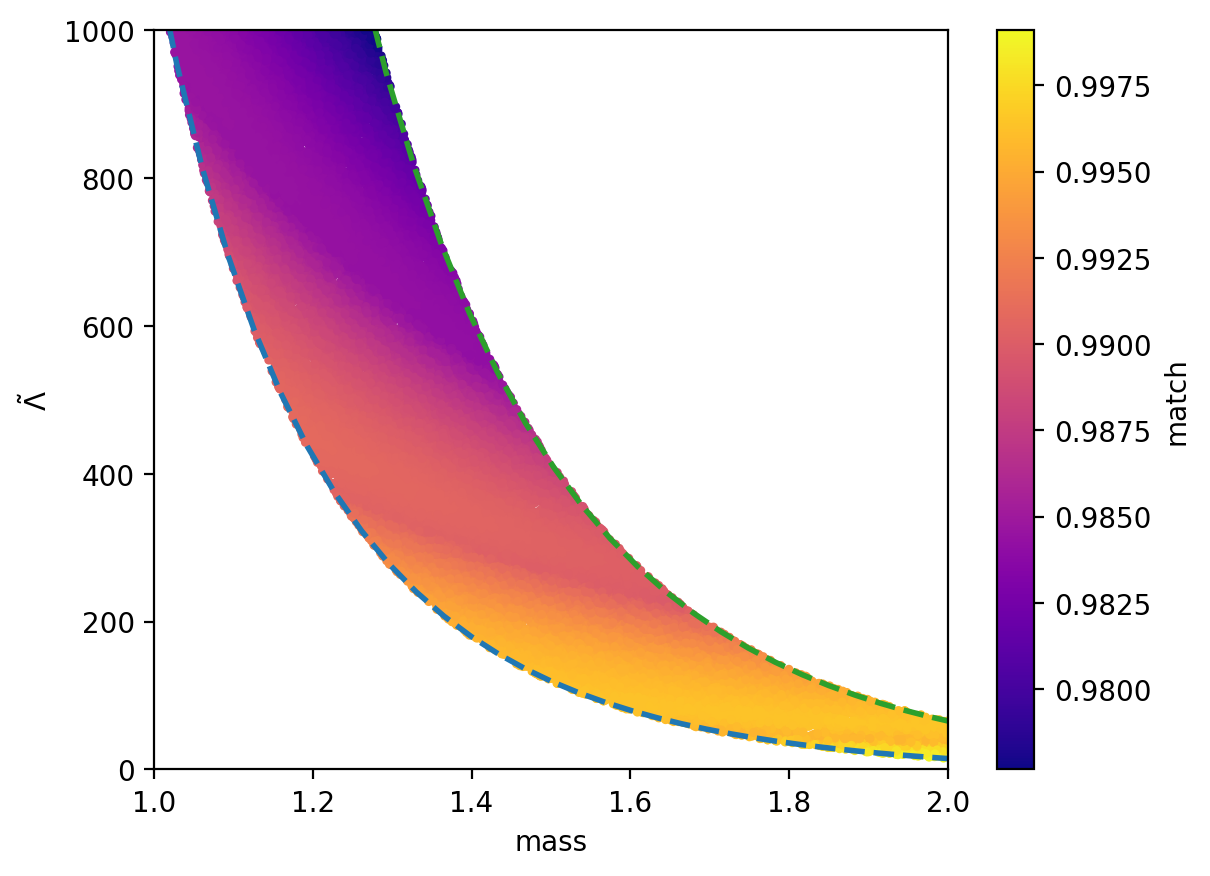
\includegraphics[width=\textwidth]{Figures/eos-meas/eos_match.png}
\caption{Match between gravitational waveforms for equal mass binaries with and without tidal deformability included. The match is calculated as the noise-weighted overlap between the two waveforms in the frequency range $20-2048$ Hz using the Advanced LIGO design sensitivity noise curve \texttt{aLIGODesignSensitivityP1200087}. Waveforms are generated using masses ranging from $1-2$\msun, and for the waveform including tidal deformability we use values of $\tilde\Lambda=\Lambda_{1}=\Lambda_{2}$ that span the range of plausible values between the soft (lower curve) and stiff (upper curve) equations of state selected for our analysis.}
\label{fig:tidal_phase}
\end{figure}

To explore the effect of a stiff or soft equation of state on our ability to place precise constraints, we select for our analysis three equations of state that span the full plausible range. We require that each equation of state support a maximum neutron star mass of 2\msun. For simplicity, we do not include any equations of state that contain a phase transition of the dense matter. The equations of state are selected from a set of 2000 that are constructed from nuclear chiral effective field theory, which is calibrated to nuclear experiments up to the nuclear saturation density. From soft to stiff, our chosen equations of state are labeled EOS 487, EOS 895, and EOS 1250, and in Figure~\ref{fig:eos_with_constraints} we show their location in the $R_{1.4}-\Lambda_{1.4}$ plane along with a selection of recent equation of state constraints from electromagnetic and gravitational-wave observations to date. Also plotted are the pairs of ($R_{1.4}$, $\Lambda_{1.4}$) values from the entire set of 2000 equations of state used in our analysis as a prior distribution for the parameter estimation, which we discuss in greater detail in Section~\ref{sec:eos_meas_pe}.

\begin{figure}[ht]
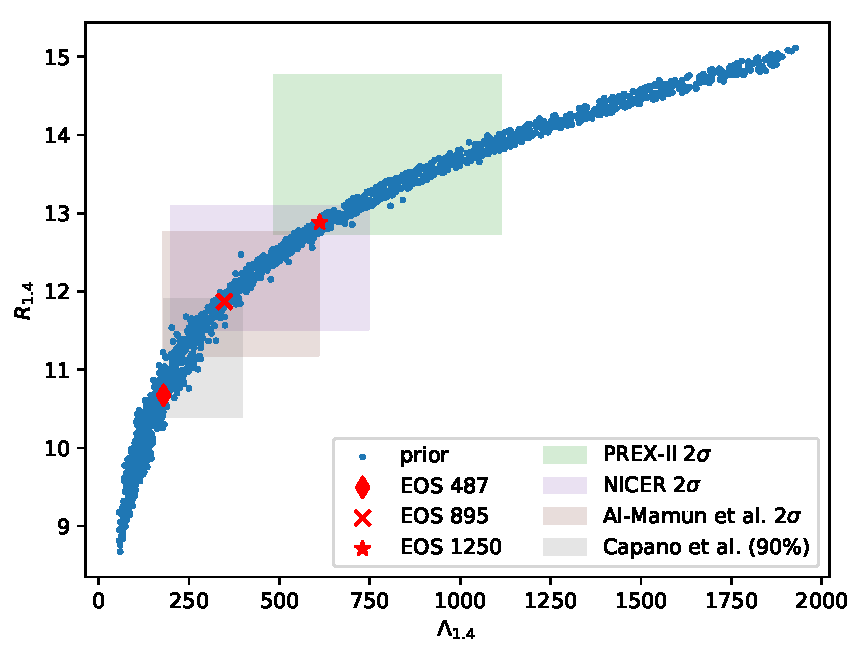
\includegraphics[width=\textwidth]{Figures/eos-meas/nsat_radius_vs_lambda.pdf}
\caption{
The radius in kilometers and dimensionless tidal deformability of a 1.4\msun\ neutron star, denoted $R_{1.4}$ and $\Lambda_{1.4}$, for the equations of state used in this work. The soft, medium, and stiff equations of state whose measurability we assess, EOS 487, EOS 895, and EOS 1250, are shown as a red diamond, red cross, and red star, respectively. The ($\Lambda_{1.4}, R_{1.4}$) coordinates for the 2000 equations of state used as a prior distribution in our analysis are shown in blue. Shaded regions represent a selection of constraints on the equation of state from gravitational-wave and electromagnetic observations, and nuclear experiment. The constraints span a significant range with potentially some tension between them. The three equations of state we investigate in this work are chosen to span the majority of the range covered by these constraints.
}
\label{fig:eos_with_constraints}
\end{figure}

\section{Parameter estimation}\label{sec:eos_meas_pe}

% Bayesian inference boilerplate
In general, under the assumption of Gaussian noise characterized by a power spectral density $S(f)$, the likelihood of obtaining detector data $d$ given the presence of a gravitational waveform $h(\theta)$ is
\begin{equation}
    \mathcal{L}(d|\theta)\propto\exp\left[-\frac{1}{2}\left<d-h(\theta)|d-h(\theta)\right>\right],
\end{equation}
where
\begin{equation}
    \left<a|b\right>=4\mathfrak{R}\int_{f_{\mathrm{min}}}^{f_{\mathrm{max}}}\frac{\tilde{a}^{*}(f)\tilde{b}(f)}{S(f)}df
\end{equation}
is the noise-weighted inner product~\cite{Finn:1992xs,Chernoff:1993th} and $\theta= \left\{ \theta_{1},\theta_{2},\ldots,\theta_{n} \right\}$ is the set of intrinsic and extrinsic parameters defining the waveform.
In evaluating this likelihood, we can obtain estimates of the gravitational-wave parameters $\theta$ through the joint posterior probability distribution
\begin{equation}
    p(\theta|d)\propto\mathcal{L}(d|\theta)p(\theta),
\end{equation}
where $p(\theta)$ is the assumed prior probability distribution of the parameters. Then the marginal posterior probability distribution for an individual parameter is obtained by integrating $p(\theta|d)$ over all nuisance parameters. For instance, the marginalized posterior distribution for $\theta_{1}$ is
\begin{equation}
    p(\theta_{1}|d)=\int p(\theta|d)~\mathrm{d}\theta_{2}\mathrm{d}\theta_{3}\ldots\mathrm{d}\theta_{n}.
\end{equation}

We use \textit{PyCBC Inference}~\cite{Biwer_2019} with the parallel-tempered version of the \texttt{emcee} sampler~\cite{Foreman_Mackey_2013,Vousden_2015,2010CAMCS...5...65G} to sample the parameter space and produce marginalized posterior distributions for the source parameters. To help speed convergence we employ the relative likelihood model available in \textit{PyCBC Inference} which uses an approximation to the full resolution likelihood near its peak in order to reduce run-time, and has been shown to produce comparable parameter estimates to non-relative models~\cite{Cornish:2010kf,Zackay:2018qdy,Finstad:2020sok}. For signals analyzed in the LIGO-Virgo network we include frequencies above a low-frequency cutoff of 20 Hz, and for Cosmic Explorer signals we use frequencies above 7 Hz. All signals are analyzed up to a high frequency cutoff of 2048 Hz.
% describe priors
We sample in source-frame component masses, component spins along the direction of the orbital angular momentum, sky location, distance, geocentric time of coalescence, inclination, polarization angle, and equation of state. For each parameter we use a prior distribution that matches the corresponding population distribution with the exception of the equation of state, where our prior distribution is made of a collection of 2000 equations of state built from nuclear theory and designed to be roughly uniform in $R_{1.4}$ over the interval $9-15$ kilometers. Each equation of state provides a mapping between mass, radius, and tidal deformability for a neutron star. At each iteration, a single equation of state is drawn and used to determine the tidal deformabilities of both neutron stars based on their source-frame masses. In generating a template waveform for the likelihood, source-frame masses are first converted to the detector frame through scaling by a factor of $(1+z)$, where $z$ is the cosmological redshift at the sampled distance assuming a flat $\Lambda$CDM cosmology. All template waveforms are generated using the \texttt{IMRPhenomD\_NRTidal} waveform in order to match the simulated signals and avoid any systematic errors arising from different implementations across waveform families.

%\subsection{Event combination}

Multiple signals $s_{1},s_{2},\ldots,s_{N}$ are considered independent of one another and thus the posterior distributions for a given parameter $\theta_{k}$ can be combined straightforwardly across all signals~\cite{DelPozzo:2013ala,Agathos:2015uaa}
\begin{equation}
    p(\theta_{k}|s_{1},s_{2},\ldots,s_{N})=p(\theta_{k})^{1-N}\prod_{i=1}^{N} p(\theta_{k}|s_{i})
\end{equation}
where we have assumed the prior $p(\theta_{k})$ is the same for all signals. 

\section{Results}\label{sec:eos_meas_results}

In order to combine measurements across an entire population, we transform the posteriors of the equation of state for all signals to posteriors of a common parameter, $R_{1.4}$. Then each signal we analyze constitutes an independent measurement of the same physical quantity, and we can combine posterior distributions across many events following the procedure outlined in the previous section. To simulate a scenario of cumulatively combining each new signal as it occurs, we combine $R_{1.4}$ posteriors one at a time to track the radius constraint (as measured by the 90\% credible interval width) as a function of the number of signals included. This also allows for a straightforward conversion to constraint over time, given a merger rate and detector network sensitivity.

% aLIGO default results
For the 321 signals in our LIGO-Virgo network analysis the combined $R_{1.4}$ constraint is shown in Figure~\ref{fig:hlv_combined} for each of the three equations of state we used. As expected, we find a hierarchy in the constraints from the three different equations of state, with a stiffer equation of state leading to a better final precision as a result of the more measurable tidal information in the signals. After combining all signals from EOS 1250, the 90\% credible interval on $R_{1.4}$ is approximately 90 meters. For the moderately stiff EOS 895 the final 90\% credible interval width is a slightly larger 130 meters. The softest equation of state in our analysis, EOS 487, produced the weakest constraint with a final 90\% credible interval of 200 meters. These credible intervals correspond to measurement precision on the true $R_{1.4}$ in each population of 0.7\%, 1.1\%, and 1.9\% respectively. 

\begin{figure}[ht]
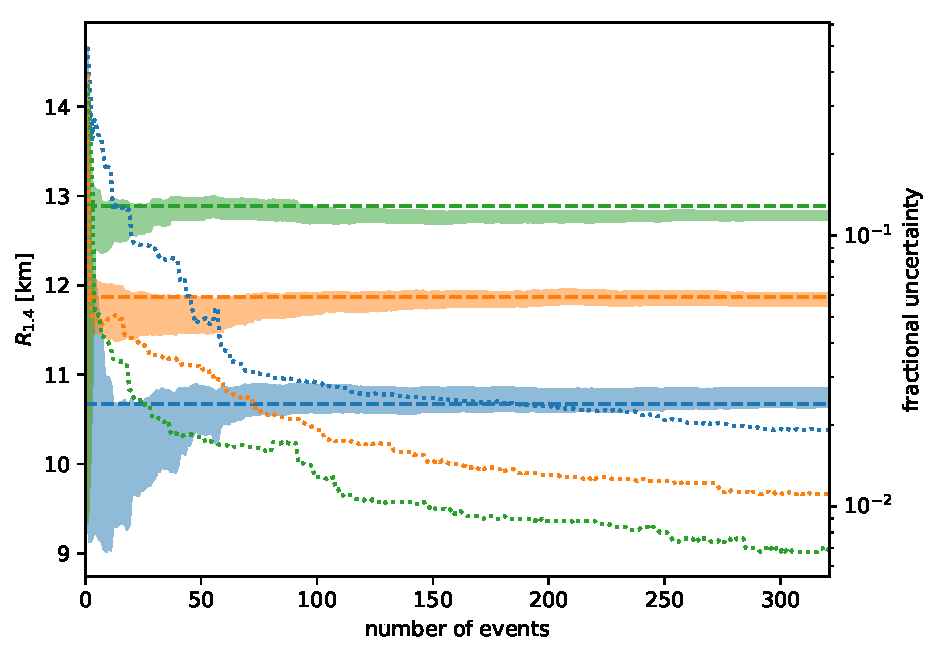
\includegraphics[width=\textwidth]{Figures/eos-meas/final_pop_hlv_combined_radius_3eos_gaussian_prior_seed0_bw0p3.pdf}
\caption{Combined $R_{1.4}$ measurements for our Gaussian mass distributed population in the LIGO-Virgo network. Results are shown for the soft (blue), medium (orange), and stiff (green) equations of state that we used. Signals are combined one at a time to show an updating constraint on the measurement as each signal is added. Shaded regions represent the 90\% credible interval for each measurement. The true values of $R_{1.4}$ for each of the equations of state are plotted as horizontal dashed lines in the appropriate color. Dotted lines show the fractional uncertainty in the measurement at each number of signals included, measured as the ratio of the 90\% credible interval to the true value of $R_{1.4}$ for a given equation of state.}
\label{fig:hlv_combined}
\end{figure}

% aLIGO default with SNR < 30
Constraints at intermediate numbers of signals will depend on the particular order in which the signals are combined, but we attempt to determine a general threshold for 10\% precision in two ways: 1. we perform the signal combination for 10 random permutations of the order; 2. we remove all signals with signal-to-noise $\rho>30$ and combine the remainder of the population to prevent any outsize influence from anomalously loud events. With both methods we find that a 10\% precision threshold is achieved after combining roughly 50 signals. This is consistent with other works that have found a better than 10\% constraint for similar numbers of signals seen by the LIGO-Virgo network~\cite{Lackey:2014fwa,Vivanco:2019qnt}. In Figure~\ref{fig:hlv_combined_snr_lt_30} we plot the result of combining the 277  signals in the population with $\rho < 30$. The final $R_{1.4}$ constraint for each of the equations of state is a factor of roughly 1.5 larger than was found for the entire population as a consequence of removing the loudest signals.

\begin{figure}[ht]
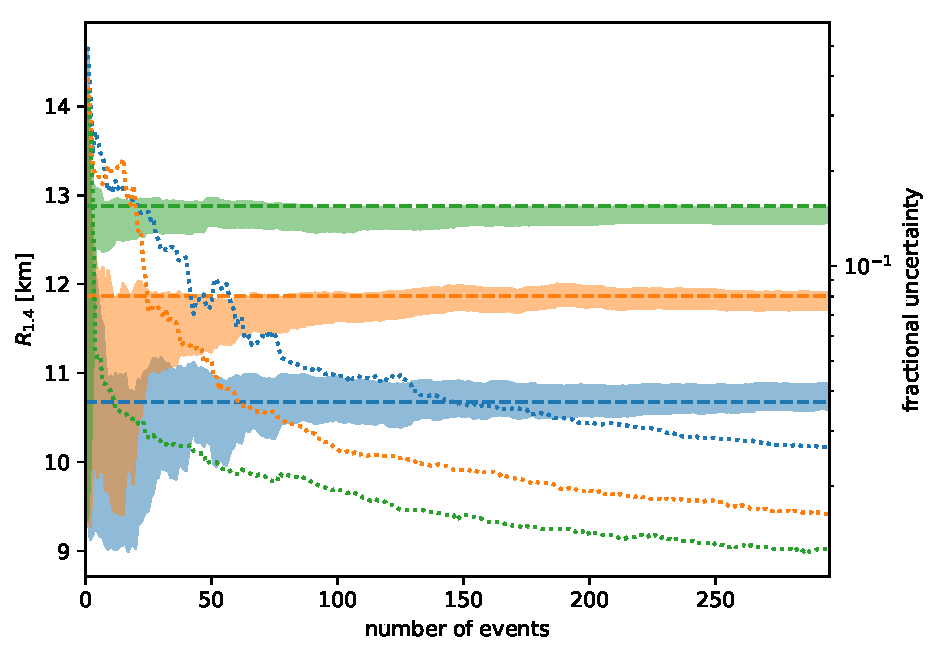
\includegraphics[width=\textwidth]{Figures/eos-meas/final_pop_hlv_combined_radius_3eos_gaussian_prior_seed0_bw0p3_snr_lt_30.pdf}
\caption{Same as Figure~\ref{fig:hlv_combined} except including only signals with signal-to-noise $\rho<30$. By removing louder signals we attempt to mitigate any potentially outsize effect on the radius constraint from signals that are unlikely to be seen by the LIGO-Virgo network. For the stiff, medium, and soft equations of state we find that a 10\% precision measurement on $R_{1.4}$ is reached after 5, 30, and 50 signals, respectively.}
\label{fig:hlv_combined_snr_lt_30}
\end{figure}

% aLIGO uniform (wrong) prior
In previous works it has been shown that imperfect knowledge of the mass distribution of neutron stars can introduce a bias into the equation of state measurement, owing to the mass dependence of the tidal deformability~\cite{Agathos:2015uaa,Wysocki:2020myz}. To investigate the implications of this effect in the context of precision equation of state measurements, we repeat our analysis on the Gaussian distributed mass population using a prior on the component masses that is uniform in the range $1-2$\msun. The combined $R_{1.4}$ constraint results from this analysis can be seen in Figure~\ref{fig:hlv_combined_uniform_prior}, where the signal ordering is the same as in Figure~\ref{fig:hlv_combined} for the sake of comparison. We find a small but significant bias toward smaller radii in our $R_{1.4}$ measurement for all three equations of state in our analysis, although the statistical uncertainties are not significantly changed. For EOS 1250 and EOS 895, we find the bias is enough to exclude the true value of $R_{1.4}$ at very high confidence after combining about 20 and 100 signals, respectively.

\begin{figure}[ht]
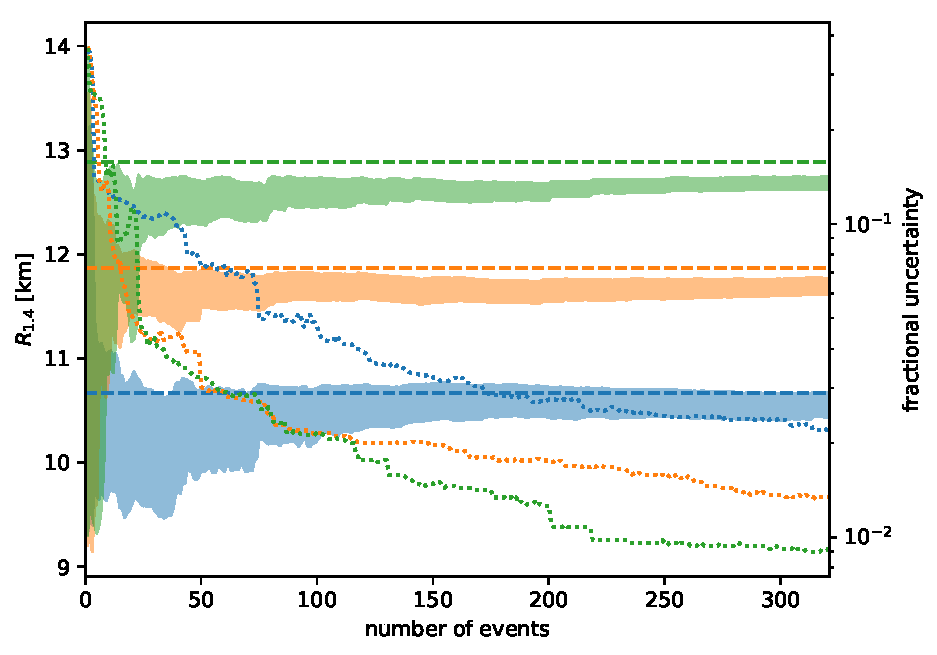
\includegraphics[width=\textwidth]{Figures/eos-meas/final_pop_hlv_combined_radius_3eos_uniform_prior_seed0_bw0p35.pdf}
\caption{Same as Figure~\ref{fig:hlv_combined} except we recover all signals with a uniform prior on the source-frame component masses from $1-2$\msun. This incorrect choice of mass prior introduces a bias in the equation of state measurement, leading to systematically lower estimates of $R_{1.4}$. We find that for EOS 1250 and EOS 895 the bias causes the true equation of state to be ruled out at high confidence after about 20 and 100 signals, respectively.}
\label{fig:hlv_combined_uniform_prior}
\end{figure}

% aLIGO uniform population
We investigate also the effect on a precision equation of state constraint from a neutron star mass distribution with greater representation of higher mass stars, since larger masses correspond to smaller $\Lambda$. To do this we perform our analysis on a population that is drawn uniformly in neutron star masses from $1-2$\msun. The combined $R_{1.4}$ constraint results are shown in Figure~\ref{fig:hlv_combined_uniform_pop}. We find for each equation of state we analyze the $R_{1.4}$ constraint is essentially unchanged from the Gaussian distributed population analysis, with final measurement precisions ranging from $1-2\%$.

\begin{figure}[ht]
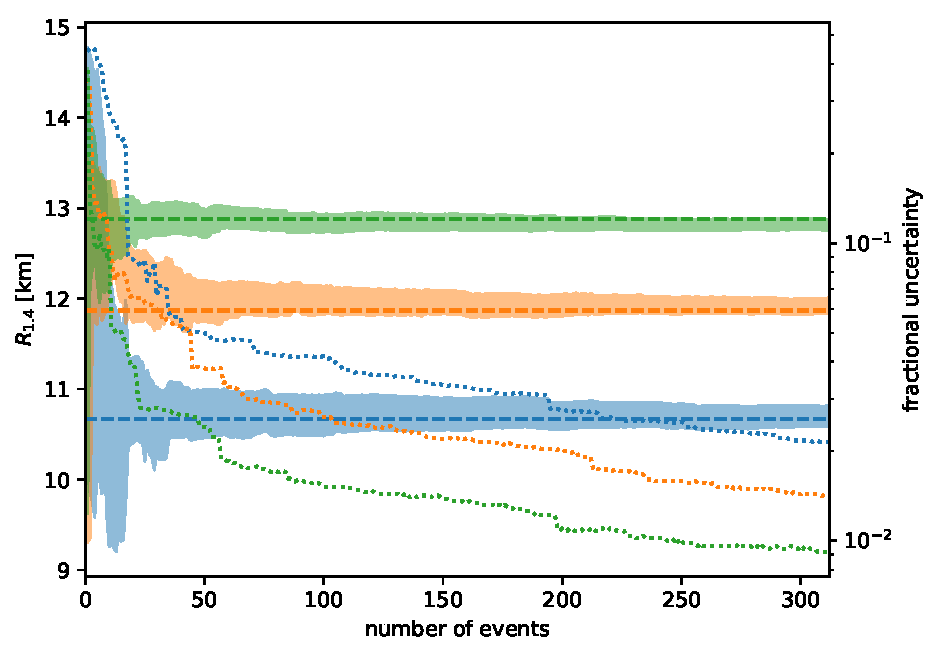
\includegraphics[width=\textwidth]{Figures/eos-meas/final_pop_hlv_combined_radius_3eos_uniform_prior_uniform_pop_seed3_bw0p3_312events.pdf}
\caption{
Combined $R_{1.4}$ measurements for our uniform mass population in the LIGO-Virgo network. Source-frame component masses are drawn from $1-2$\msun\ to represent a population with more high-mass neutron stars. All signals are recovered with a uniform mass prior from $1-2$\msun\ and signals are combined following the same procedure as the Gaussian mass population. We find the combined equation of state measurements from the uniform mass population are essentially unchanged from the Gaussian mass population, with precision on the measurement of $R_{1.4}$ ranging from $1-2\%$. 
}
\label{fig:hlv_combined_uniform_pop}
\end{figure}

% aLIGO probability of seeing events
While our LIGO-Virgo analysis includes hundreds of binary neutron star signals to produce a combined constraint, it is not at all certain that the merger rate and detector sensitivity will produce so many signals. To convert our signal-number forecast to a potential time horizon, we estimate the probability of seeing different numbers of events, assuming any population of mergers in the local universe will follow the universal analytic signal-to-noise distribution described in \cite{Chen:2014yla}. We calculate this probability as a function of the total number of events, and we convert that to number of years at the projected sensitivity for the upcoming fourth LIGO observing run (O4). We use the median binary neutron star merger rate estimate $\mathcal{R}=320~\mathrm{Gpc}^{-3}\mathrm{yr}^{-1}$ from \cite{Abbott:2020gyp}, the projected O4 search volume $VT=0.016~\mathrm{Gpc}^{3}\mathrm{yr}$ from \cite{Aasi:2013wya}, and we assume a detection threshold network signal-to-noise $\rho_{t}=9$. The calculated probabilities of seeing 10, 25, and 50 events with $\rho > 10$, consistent with the signals we include in this work, can be seen in Figure~\ref{fig:prob_of_events}. We note that O4 is expected to last approximately one year, though we calculate probabilities beyond that timeline to allow for any delays in the planned detector upgrades and to provide a lower limit for future observing runs that are expected to operate with improved sensitivity. We find that while 10 binary neutron star signals with $\rho>10$ will almost certainly be seen in just 3 years of observation at O4 sensitivity, it will take over 12 years at this sensitivity to have any significant probability of seeing 50 signals.

\begin{figure}[ht]
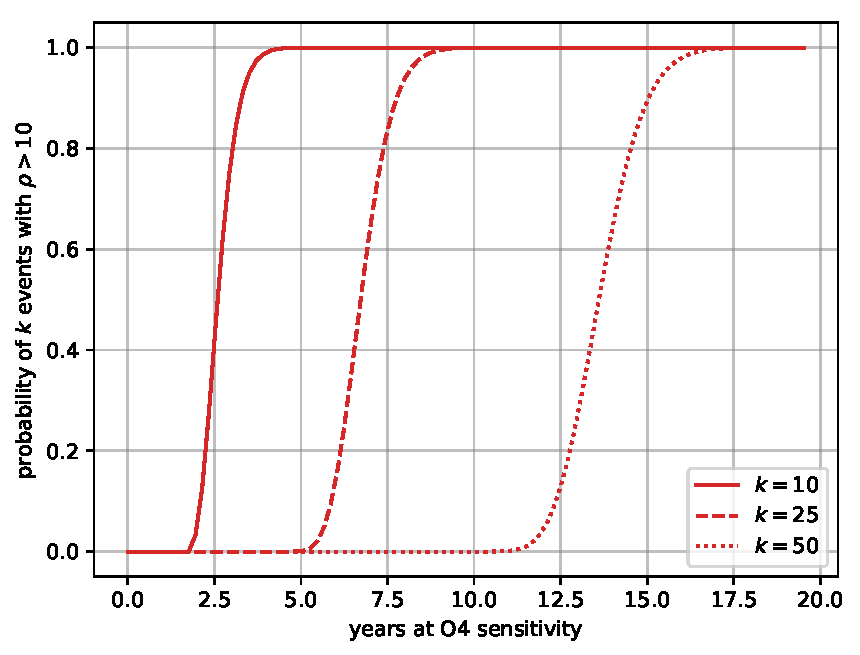
\includegraphics[width=\textwidth]{Figures/eos-meas/probability_over_time_snr10.pdf}
\caption{Probability of seeing 10, 25, and 50 events with signal-to-noise $\rho>10$ over time, assuming the population of merging binary neutron stars in the local universe follows the universal signal-to-noise distribution described in~\cite{Chen:2014yla}. The probabilities for 10, 25, and 50 events are shown as solid, dashed, and dotted lines, respectively. We use the median binary neutron star merger rate estimate from \cite{Abbott:2020gyp} and the projected sensitive volume for the upcoming fourth observing run (O4) of the Advanced LIGO network~\cite{Aasi:2013wya} to plot probabilities against number of years at O4 sensitivity. We assume a detection threshold network signal-to-noise ratio of 9.}
\label{fig:prob_of_events}
\end{figure}

Planned upgrades are expected to substantially increase detector sensitivity for the fifth observing run and beyond, though no official estimate of the search volume has yet been published. An improved network sensitivity would effectively shift the probability curves in Figure~\ref{fig:prob_of_events} leftward by the factor of improvement in search volume, though we note that even an order of magnitude improvement would likely result in at most 50 signals in several years of observation under the assumptions made here.

% CE default result
Finally, we explore the ability of Cosmic Explorer to precisely measure the equation of state. The extreme sensitivity of the Cosmic Explorer design means that it is expected to be sensitive to the complete population of merging binaries out to a redshift of $z=1$~\cite{CEHS}. This means that given current merger rate estimates, Cosmic Explorer will likely see hundreds of binary neutron star signals with $\rho>100$ in a single year of observation, and our simulated population of 335 signals is approximately representative of that set. The combined $R_{1.4}$ constraint for EOS 487 and EOS 895 are shown in Figure~\ref{fig:ce_combined}. We find that for both equations of state a 10\% precision threshold is achieved almost immediately, with the precision improving to 0.6\% and 0.15\% after combining all signals for EOS 487 and EOS 895, respectively. We also note that these constraint projections are likely slight overestimates, as there will be many more signals with $\rho<100$ seen in one year of observation that would still contain measurable tidal information. While the combined equation of state measurement will almost certainly be dominated by the louder signals we consider here, it is possible that quieter signals will contribute to improve the constraint somewhat.

\begin{figure}[ht]
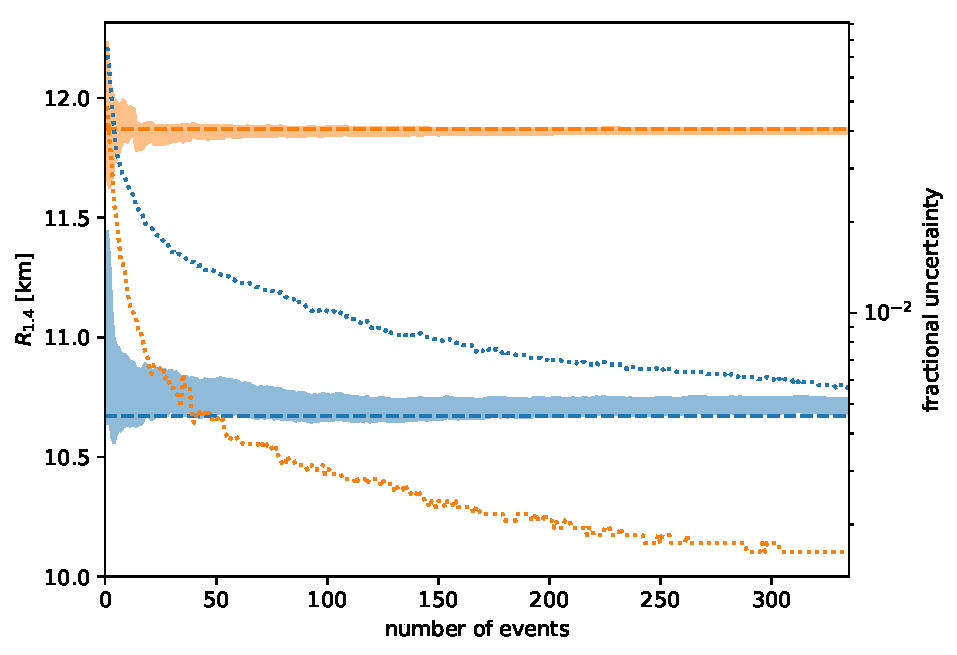
\includegraphics[width=\textwidth]{Figures/eos-meas/final_pop_ce_combined_radius_3eos_gaussian_prior_seed1_bw0p3.pdf}
\caption{
Combined $R_{1.4}$ measurements for our Gaussian mass distributed population in Cosmic Explorer, which is representative of the signals expected in one year of observation. Results are shown for the soft (blue) and medium (orange) equations of state in our analysis. As in Fig.~\ref{fig:hlv_combined} the horizontal dashed lines indicate the true value of $R_{1.4}$ for each equation of state, and the dotted lines show the calculated fractional uncertainty which is defined as the ratio of the 90\% credible interval to the true value of $R_{1.4}$. We find that for both equations of state, a 10\% precision threshold on the measurement of $R_{1.4}$ is achieved almost immediately, consistent with the third-generation detector result from~\cite{Pacilio:2021jmq}. The measurement precision improves to 0.6\% and 0.15\% for the soft and medium equations of state, respectively, after all signals are combined.
}
\label{fig:ce_combined}
\end{figure}

% CE uniform (wrong) prior result
We also check whether the Cosmic Explorer constraints are robust to an incorrect choice of mass prior by repeating the analysis using a uniform mass prior from $1-2$\msun. Systematic biases from an incorrect choice of prior are smaller for louder signals, so we expect that our population of Cosmic Explorer signals will suffer less from this effect. Figure~\ref{fig:ce_combined_uniform} shows the combined $R_{1.4}$ constraints from this analysis for the medium and soft equations of state we investigated, where again the ordering has been preserved from Figure~\ref{fig:ce_combined} to allow easy comparison. We find there is again a bias toward smaller radii for both EOS 487 and EOS 895, though it is much smaller in absolute terms than that seen in the LIGO-Virgo analysis. Still, the correspondingly smaller statistical uncertainties on our combined measurements make it so the true $R_{1.4}$ values lie right at the upper boundary of the 90\% credible interval for both equations of state, emphasizing the need for a good estimate of the neutron star mass distribution even for Cosmic Explorer. As was the case in our LIGO-Virgo analysis, we find the statistical uncertainties on the combined measurements are largely unchanged from the Gaussian mass prior analysis.

\begin{figure}[ht]
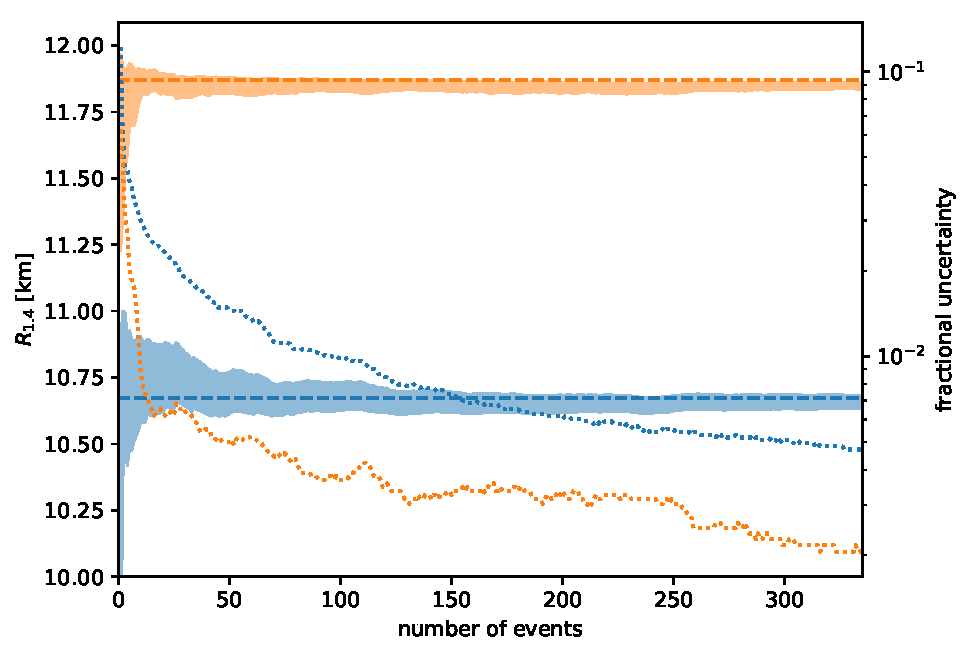
\includegraphics[width=\textwidth]{Figures/eos-meas/final_pop_ce_combined_radius_3eos_uniform_prior_seed1_bw0p3.pdf}
\caption{Same as Figure~\ref{fig:ce_combined} except we recover signals using a uniform mass prior from $1-2$\msun. The ordering of signals has been preserved from the Gaussian prior analysis for comparison, and it can be seen that the combined constraints for both equations of state is again biased toward smaller radii as a result of the incorrect mass prior. The bias is smaller than what was seen in our LIGO-Virgo analysis as a result of the much louder signals in the Cosmic Explorer population, however the true values for both equations of state are still found at the edge of their respective 90\% credible interval because of the correspondingly smaller statistical uncertainties on these measurements.}
\label{fig:ce_combined_uniform}
\end{figure}

\section{Conclusion}\label{sec:eos_meas_conclusion}
We  presented an updated forecast using more plausible equations of state for  binary neutron star mergers seen  by a LIGO-Virgo network, and new results for the proposed Cosmic Explorer detector. We use the most up-to-date estimates for the range of plausible equations of state and of the merger rate in the local universe. We find that Advanced LIGO will constrain $R_{1.4}$ to within 10\% at 90\% confidence with the first 50 signals, largely consistent with previous works, and we show that this projection is robust to a change in the mass population of neutron stars. We also extend the projection to find that across the full range of plausible equations of state, Advanced LIGO will be able to measure $R_{1.4}$ to better than about 2\% after 321 signals, although the probability of seeing this many signals before third generation detectors become operational is potentially  very low. On the other hand we find that the much greater sensitivity of Cosmic Explorer means it will be able to measure $R_{1.4}$ to better than 0.6\% at 90\% confidence across the full range of plausible equations of state with one year of observation. This precision from Cosmic Explorer will be sufficient to distinguish even similarly soft equations of state from one another at high confidence.

% mass prior effect
As discussed by Wysocki {\it et al.}, our analysis confirms that accurate knowledge of the mass distribution of neutron stars in the population of merging binaries is vital to making an unbiased measurement of the equation of state. We find that biases due to an incorrect mass prior can be present even in measurements from a population of loud signals in a third-generation detector like Cosmic Explorer, and as such we emphasize the added importance of efforts to mitigate these biases in the context of precision equation of state measurements.



